% =================================================================
%  DSC 208R — Data Management for Analytics
%  Task Parallelism: Comprehensive Review
%  Source slides: “Data Engineering for Machine Learning – Task parallelism”
% =================================================================
\documentclass[11pt]{article}

% -------------------- Packages --------------------
\usepackage[utf8]{inputenc}
\usepackage{amsmath,amssymb,amsfonts}
\usepackage{graphicx}
\usepackage{booktabs}
\usepackage{tikz}
\usetikzlibrary{positioning}   % for 'right=of', 'below=of', etc.
\usepackage{pgfplots}
\usepackage{enumitem}
\usepackage{listings}
\usepackage{hyperref}
\usepackage{caption}
\pgfplotsset{compat=1.17}

% -------------------- Listings --------------------
\lstset{
  basicstyle=\ttfamily\small,
  keywordstyle=\bfseries,
  commentstyle=\itshape,
  showstringspaces=false,
  frame=single,
  breaklines=true
}

% -------------------- Document --------------------
\begin{document}

\begin{center}
  {\LARGE\bfseries Task Parallelism}\\[2mm]
  {\large Comprehensive Review}\\[1mm]
  {\normalsize DSC 208R — Parallel Data Processing and the Cloud}
\end{center}
\vspace{-0.6em}\hrule\vspace{0.9em}

\tableofcontents
\newpage

% ================================================================
\section{Motivation and Big Picture}

\paragraph{Divide \& Conquer.}  
Task parallelism applies the classical divide-and-conquer strategy to data-engineering workloads: \emph{place different tasks on different workers}; if they need the same dataset, simply \emph{replicate} it to every worker:contentReference[oaicite:0]{index=0}.  

This idea is attractive when:  

\begin{itemize}[itemsep=0pt]
  \item The task graph exposes substantial concurrency.
  \item The dataset is not too large to replicate across workers.
  \item Tasks are heterogeneous (e.g., feature engineering $\rightarrow$ model training $\rightarrow$ evaluation).
\end{itemize}

% ================================================================
\section{Core Concepts of Task Parallelism}

\subsection{Task Graphs and Topological Scheduling}

Workloads are represented as Directed Acyclic Graphs (DAGs) of tasks.  
A scheduler performs a \emph{topological sort} to respect dependencies when assigning tasks to workers:contentReference[oaicite:1]{index=1}.

\subsection{Workers and Threads}

A “worker” may be a whole node (process-level parallelism) or a single CPU core (thread-level parallelism).  For example, Dask can treat a 4-node cluster with 4 cores each as 16 total workers:contentReference[oaicite:2]{index=2}.

\subsection{Pros and Cons}

\begin{itemize}[itemsep=0pt]
  \item \textbf{Pros:} Simple mental model; independent workers imply low software complexity.:contentReference[oaicite:3]{index=3}
  \item \textbf{Cons:} Data replication wastes memory/storage; workers may sit idle when concurrency drops.:contentReference[oaicite:4]{index=4}
\end{itemize}

% ================================================================
\section{Degree of Parallelism}

\begin{quote}
\emph{“The largest amount of concurrency possible in the task graph; i.e., how many tasks can run simultaneously.”}:contentReference[oaicite:5]{index=5}
\end{quote}

In the illustrative DAG (Figure \ref{fig:dag}), the degree of parallelism is 3; hence deploying more than three workers yields no additional speed-up.

\begin{figure}[h]
  \centering
  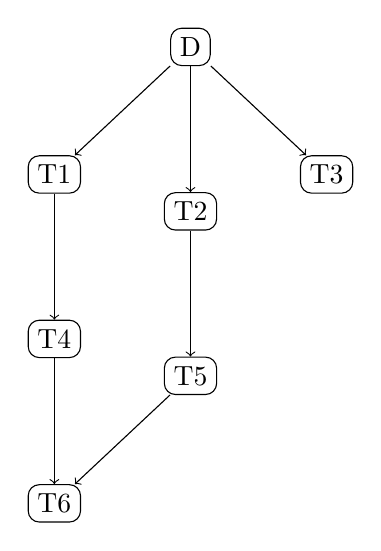
\begin{tikzpicture}[node distance=1.6cm, every node/.style={draw,rounded corners}]
    \node (d)  {D};
    \node (t1) [below left=of d]  {T1};
    \node (t2) [below=of d]       {T2};
    \node (t3) [below right=of d] {T3};
    \node (t4) [below=of t1]      {T4};
    \node (t5) [below=of t2]      {T5};
    \node (t6) [below=of t4]      {T6};

    \foreach \a/\b in {d/t1,d/t2,d/t3,t1/t4,t2/t5,t4/t6,t5/t6}
      \draw[->] (\a) -- (\b);
  \end{tikzpicture}
  \caption{Example task graph with maximum concurrency of 3.}
  \label{fig:dag}
\end{figure}

% ================================================================
\section{Mathematical Formulations}

\subsection{Speed-Up}

\[
\text{Speed-up}(n)=
\frac{\text{Completion time with 1 worker}}
     {\text{Completion time with $n$ workers}}\;.
\]
Ideal (linear) speed-up equals $n$.  Real workloads often attain sub-linear speed-up due to limited degree of parallelism, data transfer, and scheduling overhead:contentReference[oaicite:6]{index=6}.

\subsection{Lower Bound on Completion Time}

The parallel completion time is lower-bounded by the \emph{longest path} (critical path) in the task graph; idle time arises whenever the ready-task set is smaller than the worker pool:contentReference[oaicite:7]{index=7}.

% ================================================================
\section{Worked Example: Six-Task Workflow on Three Workers}

Using the durations from the slides (in seconds):

\[
\text{T1}=10,\;
\text{T2}=5,\;
\text{T3}=15,\;
\text{T4}=5,\;
\text{T5}=20,\;
\text{T6}=10.
\]

\subsection{Serial vs.\ Parallel Runtime}

\begin{itemize}[itemsep=0pt]
  \item Serial runtime: $10+5+15+5+20+10 = 65\,$s.:contentReference[oaicite:8]{index=8}
  \item Parallel runtime (three workers): $35\,$s (see Gantt chart, Figure \ref{fig:gantt}).:contentReference[oaicite:9]{index=9}
\end{itemize}

Hence speed-up $=65/35\approx1.9$, well below the ideal $3\times$.

\begin{figure}[h]
  \centering
  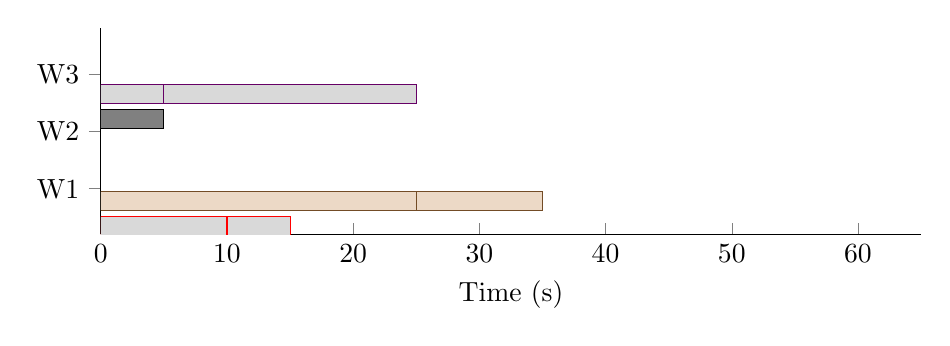
\begin{tikzpicture}
    \begin{axis}[
      xbar,
      width=12cm,
      height=4.2cm,
      xmin=0,xmax=65,
      yticklabels={W1,W2,W3},
      ytick={0.5,1.5,2.5},
      xlabel={Time (s)},
      bar width=7pt,
      axis y line*=none,
      axis x line*=bottom,
      enlarge y limits=0.4
    ]
      % worker 1
      \addplot+[fill] coordinates {(0,0.5) (10,0.5) (10,0.5)};
      \addplot+[fill=gray!30] coordinates {(10,0.5) (15,0.5)};
      \addplot+[fill] coordinates {(25,0.5) (35,0.5)};
      % worker 2
      \addplot+[fill] coordinates {(0,1.5) (5,1.5)};
      \addplot+[fill=gray!30] coordinates {(5,1.5) (25,1.5)};
      % worker 3
      \addplot+[fill] coordinates {(0,2.5) (15,2.5)};
    \end{axis}
  \end{tikzpicture}
  \caption{Illustrative Gantt chart: grey bars denote idle periods.}
  \label{fig:gantt}
\end{figure}

\paragraph{Why only 1.9×?}  
Idle periods (grey) and the critical-path bound cap attainable speed-up.  Adding more than three workers would \emph{not} reduce runtime because the degree of parallelism is already saturated.

% ================================================================
\section{Algorithm Outline: Task-Parallel Scheduler}

\begin{enumerate}[itemsep=0pt]
  \item Perform a topological sort to identify ready tasks.
  \item When a worker becomes free, assign it any ready task (FIFO, LIFO, or cost-aware heuristic).
  \item Upon task completion, mark successors as ready; repeat until all tasks finish.
  \item Optionally release idle workers early to save cloud costs when no further tasks can be assigned.:contentReference[oaicite:10]{index=10}
\end{enumerate}

% ================================================================
\section{Practical Guidelines}

\begin{itemize}[itemsep=0pt]
  \item Match the number of workers to the workload’s maximal degree of parallelism; more workers waste resources.
  \item Minimize replication overhead by keeping datasets small or by partitioning read-only reference data.
  \item Use frameworks like \emph{Dask} to exploit thread-/process-level pools automatically (e.g., 4 nodes × 4 cores = 16 workers).:contentReference[oaicite:11]{index=11}
  \item Monitor idle time; consider elastic autoscaling to decommission idle workers and cut cloud costs.
\end{itemize}

% ================================================================
\section{Future Directions}

\begin{itemize}[itemsep=0pt]
  \item Integrate critical-path analysis with cost-based schedulers for cloud cost minimization.
  \item Explore hybrid task/data-parallel approaches to reduce replication while retaining independence.
  \item Improve predictive autoscaling policies that release idle workers without hurting completion time.
\end{itemize}

% ================================================================
\section*{Conclusion}

Task parallelism offers a simple yet powerful way to accelerate data-science pipelines by exploiting concurrency in task graphs.  Its benefits, however, are bounded by degree of parallelism, data replication costs, and critical-path latency.  Careful scheduling and resource sizing are essential to approach optimal performance.

\end{document}
